\documentclass{article}

\usepackage{graphicx, caption, subcaption, amsmath, amsfonts}

\usepackage{hyperref}
\hypersetup{
    colorlinks,
    citecolor=black,
    linkcolor=black,
    urlcolor=blue
}

% Automatic float-barrier around subsections
\usepackage[section]{placeins}
\makeatletter
\AtBeginDocument{%
  \expandafter\renewcommand\expandafter\subsection\expandafter{%
    \expandafter\@fb@secFB\subsection
  }%
}
\makeatother

\setcounter{tocdepth}{2}

\begin{document}

\title{A Gentle Introduction to Elliptic Curve Cryptography}
\author{Tanner Prynn}
\maketitle

\tableofcontents
\clearpage

\section*{Foreword}
\addcontentsline{toc}{section}{Foreword}
Draft of project for Math 415B.

Status of code: complete. See \texttt{curve25519.rb}.

Status of problems: incomplete. See \texttt{problems.pdf}.

Status of report: incomplete. Outline completed with some sections filled in.

In writing this report, I aimed to hit the most important points for a picture of elliptic curves as they would be applied for cryptography. 
Some sections are (or will be) rigorous while others simply provide an overview or guided discussion of ``why things are the way they are''. 
The references provide a much more in-depth discussion of this topic.

Sections I've omitted that I could include: Projective Geometry, Finite Field Arithmetic, Derivation of Group Law for Montgomery Curves

Sections I've included that I could omit: Normal Forms for Elliptic Curves/Acceptable Changes of Variables, Pohlig-Hellman Algorithm

\clearpage

\section{Elliptic Curves}
An \textbf{elliptic curve} is a set of points satisfying an equation of the form
$$y^2 = x^3 + ax + b$$
for coefficients $a,b$ and variables $x,y$ in some field $F$ (of characteristic not 2 or 3). 
We place one additional restriction on an elliptic curve, which is that
$4a^3 + 27b^2 \neq 0$.
This condition ensures that the curve is \textit{non-singular}, which allows us to find a tangent line to any point on the curve \cite[$\S$3.1]{ecc-guide}.

Let's start with a few examples of curves, plotted over the real numbers.
Figure \ref{fig:ec-plot} shows a simple elliptic curve.
It has three real roots, which correspond to the zeroes of the polynomial $x^3 - 3x + 1$.
Figure \ref{fig:ec-plot2} shows the elliptic curve $y^2 = x^3 - 2x + 2$, which only has one real root.

\begin{figure}[h]
\centering
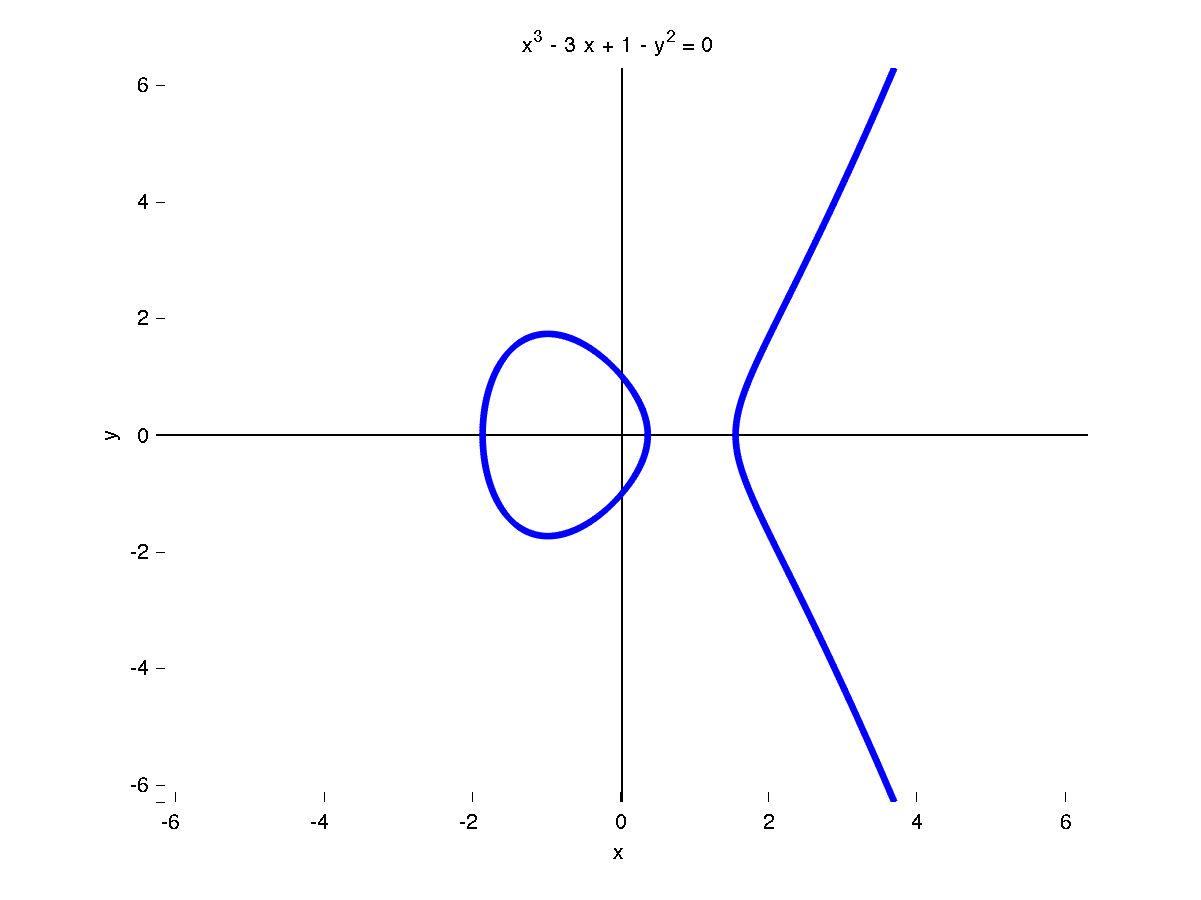
\includegraphics[width=\textwidth]{images/ec1.png}
\caption{The elliptic curve $y^2 = x^3 - 3x + 1$}
\label{fig:ec-plot}
\end{figure}

\begin{figure}[h]
\centering
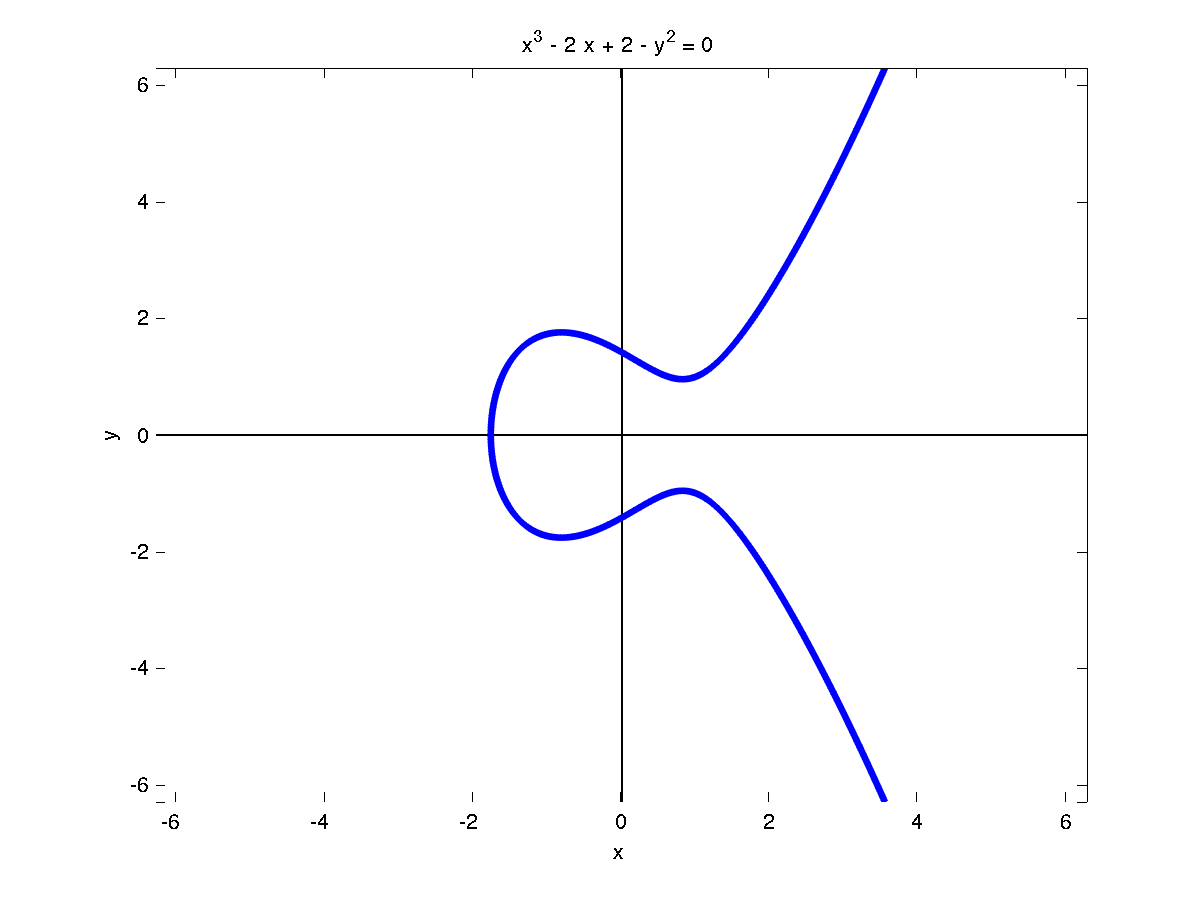
\includegraphics[width=\textwidth]{images/ec4g.png}
\caption{The elliptic curve $y^2 = x^3 - 2x + 2$}
\label{fig:ec-plot2}
\end{figure}

Figure \ref{fig:ec-singular} shows two singular curves.
To define a group operation on the points of the curve, we need to be able to take a tangent line to each point.
So we avoid these cases with that additional restriction on the coefficients.

\begin{figure}[h]
\centering

\begin{subfigure}{.5\textwidth}
	\centering
	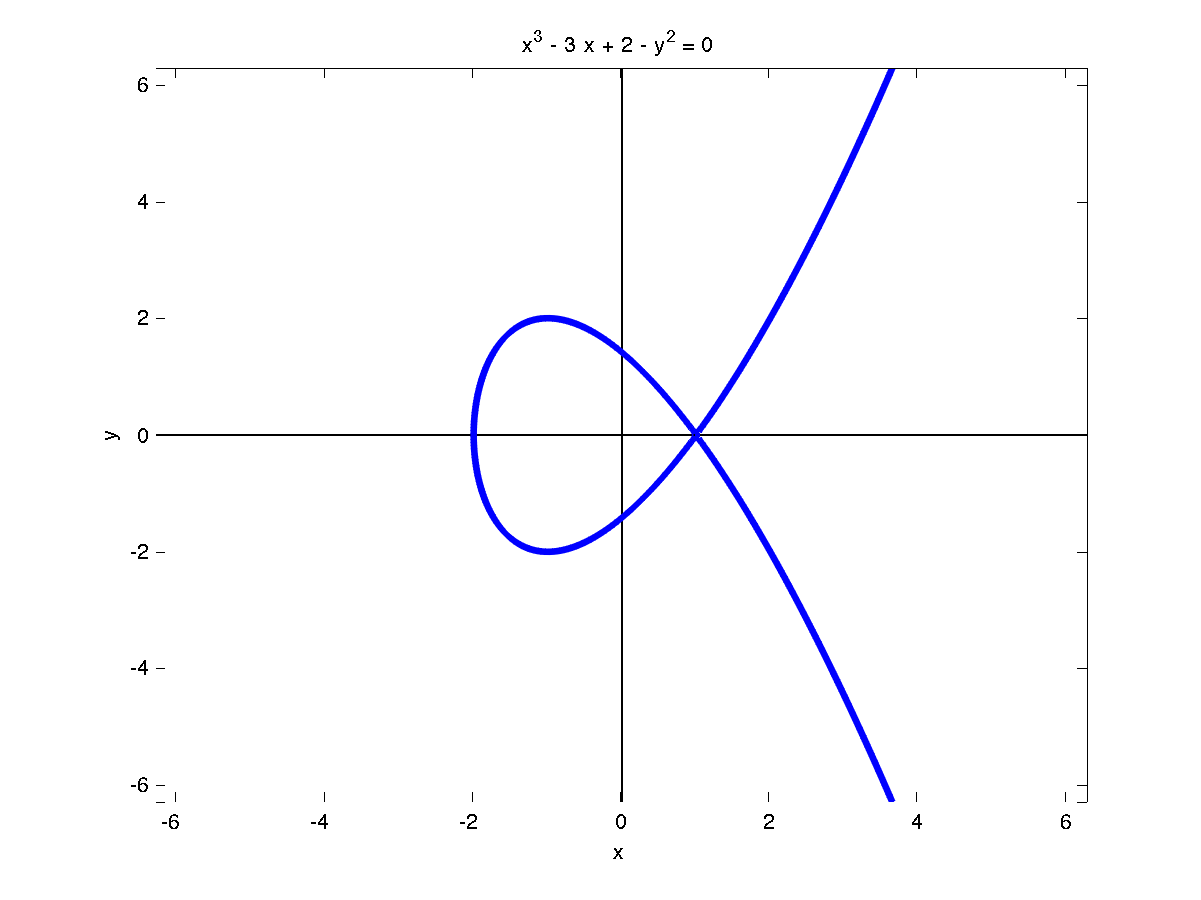
\includegraphics[width=1\linewidth]{images/ec2.png}
	\caption{The curve $y^2 = x^3 - 3x + 2$}
\end{subfigure}%
~%
\begin{subfigure}{.5\textwidth}
	\centering
	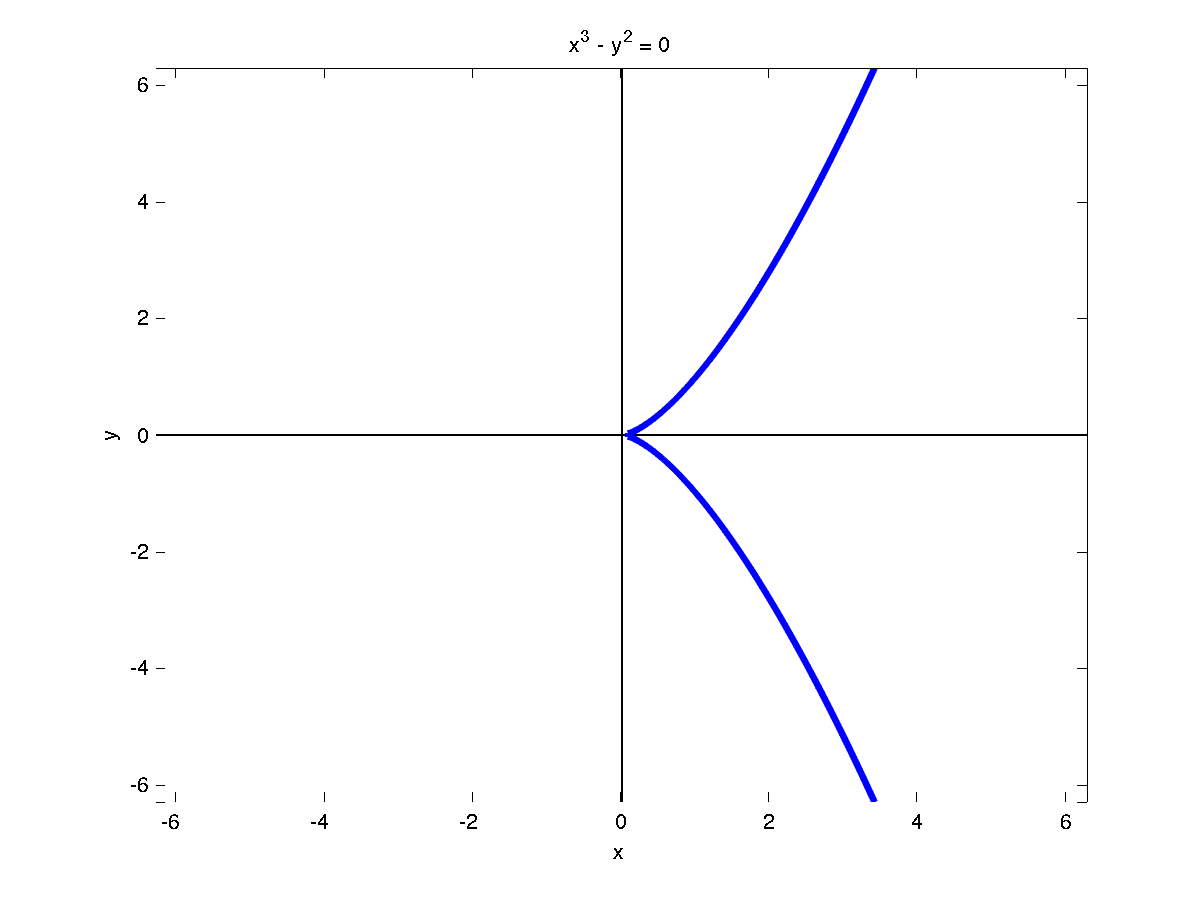
\includegraphics[width=1\linewidth]{images/ec3.png}
	\caption{The curve $y^2 = x^3$}
\end{subfigure}

\caption{These curves have a `singularity': a point where the tangent is not clearly defined.}
\label{fig:ec-singular}
\end{figure}

\subsection{Defining a Group Operation}
Now, we have an equation for a curve, and we can define the set of points 
$$C = \{(x,y) \mid x,y \in F \text{ and } y^2 = x^3 + ax + b\}$$
which is a subset of of the plane $F^2$.
We want to make the set $C$ into a group, so we need to define an operation on it.
Let's call that operation $*$, and we'll define $P_1 * P_2$ as the third intersection of the line through $P_1$ and $P_2$ which lies on the curve $C$.
Figure \ref{fig:ec-3rd-intersection} shows this operation for the simple case of two different points.

\begin{figure}[h]
\centering
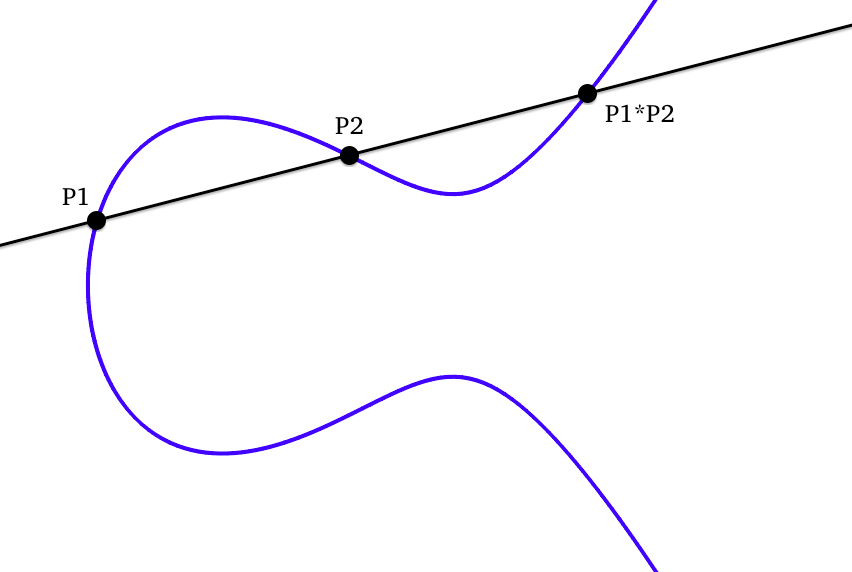
\includegraphics[width=0.6\textwidth]{images/ec4-star.png}
\caption{Finding the third point of intersection on the curve $y^2 = x^3 - 2x + 2$}
\label{fig:ec-3rd-intersection}
\end{figure}

What other cases are there?
First, we need to define $*$ when $P_1 = P_2$.
We want to have the line through $P_1$ hit the curve at exactly two points, $P_1$ and $P_1*P_1$.
To achieve this, let the line through $P_1$ be the tangent to the curve.
Then the tangent line intersects the curve at one additional point, as desired (figure \ref{fig:ec-tangent}) \cite[$\S$I.2]{rational-points}.

\begin{figure}[h]
\centering
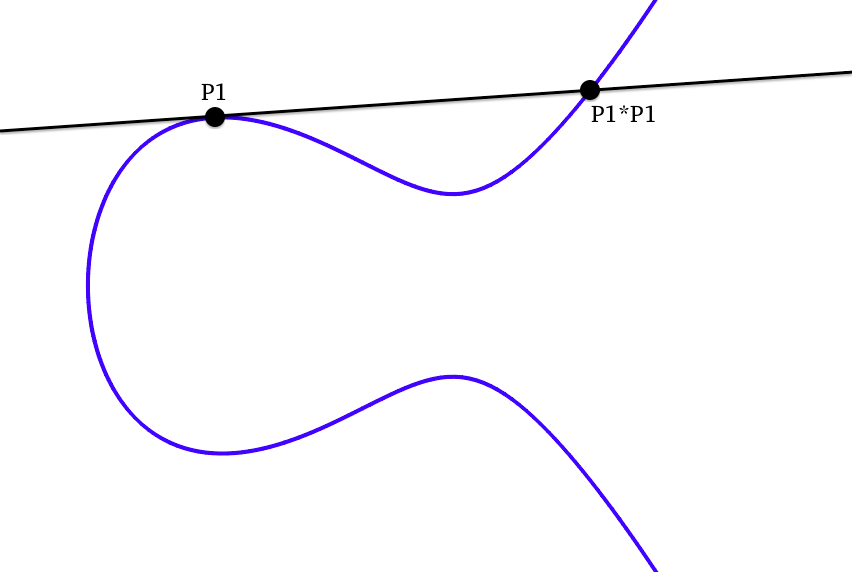
\includegraphics[width=0.6\textwidth]{images/ec4-tangent.png}
\caption{A tangent line intersects the curve at two points.}
\label{fig:ec-tangent}
\end{figure}

Now, we come to the case of a vertical line.
A vertical line will intersect our curve at exactly two points, because the curve is symmetric over the $x$-axis.
But those two points will violate our $*$ operation, because there isn't a third-point where the line intersects the curve (figure \ref{fig:ec-infinity}).
This leads us to take an idea from projective geometry: that there is an extra point on the curve called the \textit{point at infinity}.

\begin{figure}[h]
\centering
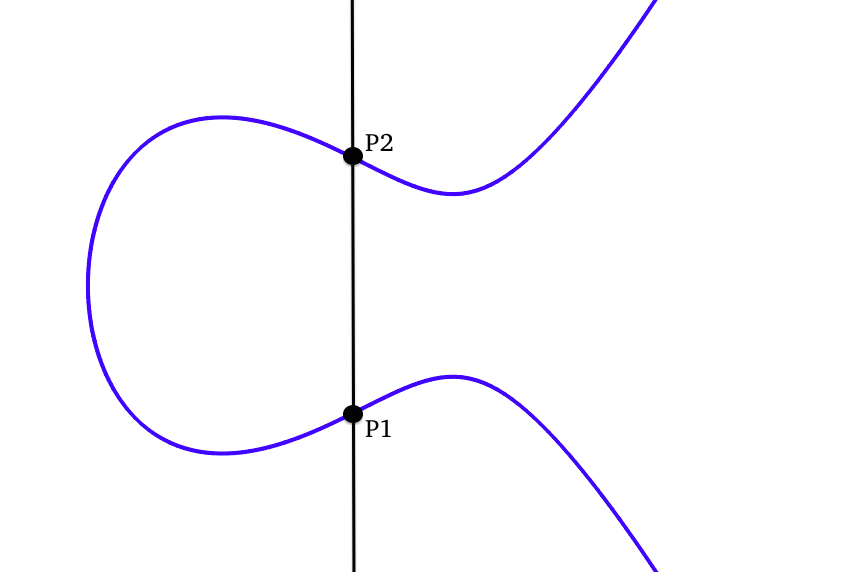
\includegraphics[width=0.6\textwidth]{images/ec4-infinity.png}
\caption{A vertical line only intersects the curve at two points.}
\label{fig:ec-infinity}
\end{figure}

The point at infinity (denoted $\infty$) is a point in the projective plane, so there isn't an intuitive way to draw it in our standard plane.
However, we can understand $\infty$ as `outside' of the plane, and simply treat it as a special geometric object.
As a benefit, we can take the third intersection of a vertical line to be $\infty$.
We then need to redefine the set of points $C$ to include $\infty$:
$$C = \{\infty\} \cup \{(x,y) \mid x,y \in F \text{ and } y^2 = x^3 + ax + b\}$$
Thus we have disposed of this problematic case \cite[$\S$2.2]{washington}.

Having $\infty$ on our curve is also useful because it is a unique point which exists on every elliptic curve.
This makes it an ideal candidate for the identity element of our group operation.
We need to redefine our operation to make this true, however.
If we reconsider the case of the vertical line, we have two points $P_1$ and $P_2$ such that $P_1 * P_2 = \infty$.
Because the curve is symmetric, all we need to do to get $P_1$ from $P_2$ is to reflect over the $x$-axis.

Let's define a new operation $+$ and say that, for any point $P \in C$, $P = P+\infty = \infty+P$.
To produce $+$ from our previous operation $*$, we only need to add one additional step: a reflection over the $x$-axis.
We will see later that this operation is commutative, which is why we chose to use the addition symbol \cite[$\S$2.2]{washington}.
Figure \ref{fig:ec-plus} revisits the previous cases to show how this new operation works.

\begin{figure}[h]
\centering

\begin{subfigure}{.5\textwidth}
	\centering
	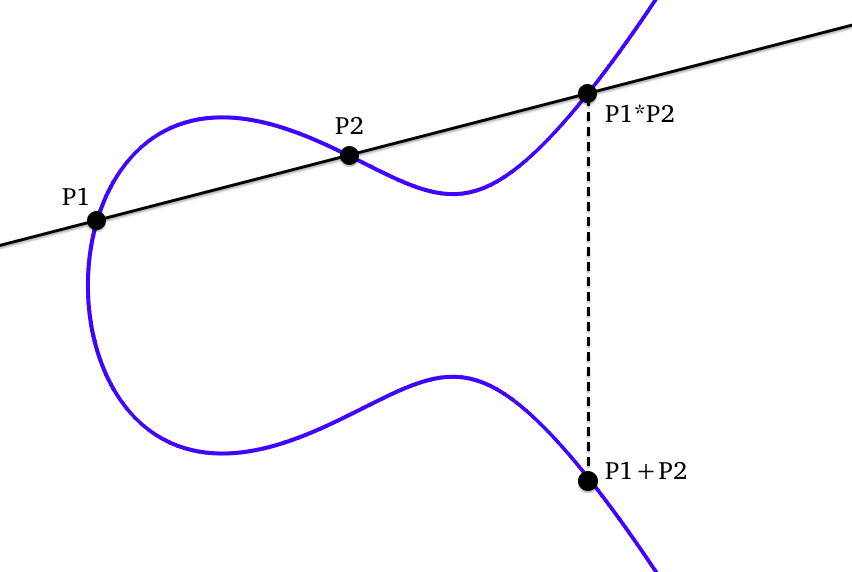
\includegraphics[width=1\linewidth]{images/ec4-plus.png}
	\label{fig:ec-plus-1}
\end{subfigure}%
~%
\begin{subfigure}{.5\textwidth}
	\centering
	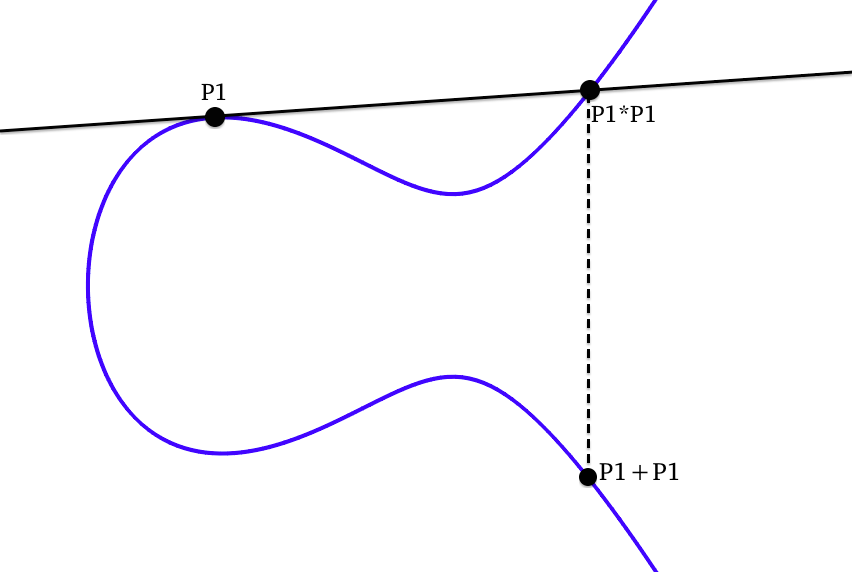
\includegraphics[width=1\linewidth]{images/ec4-plus-tangent.png}
	\label{fig:ec-plus-2}
\end{subfigure}

\caption{The $+$ operation for two points on an elliptic curve}

\label{fig:ec-plus}
\end{figure}

\subsection{Deriving the Group Law}
Now that we have defined the group operation geometrically, we can derive a formula for it.

\subsubsection{Identity}
Define $\infty$ to be the identity. For any point $P$ on $C$, $P+\infty = \infty + P = P$.

\subsubsection{Addition}
Let $P_1 = (x_1,y_1), P_2 = (x_2,y_2)$ on $C$ with $P_1 \neq P_2$.
If $x_1 = x_2$, then the line is vertical and we define $P_3 = \infty$.
Otherwise, the equation of the line through $P_1$ and $P_2$ has the form $y = mx + b$, where $m = \frac{y_2-y_1}{x_2-x_1}$ and $b = y_1 - mx_1$.
Now substitute this into the equation of our curve to obtain
$$(mx+b)^2 = x^3 + ax + b$$
Expand and rewrite to get a cubic equation in $x$
$$0 = x^3 - m^2x^2 + (a-2mb)x + b - b^2$$
We know that this equation has three roots (of which we know two), so it must be equal to
$$0 = (x-x_1)(x-x_2)(x-x_3)$$
Multiplying out, we find that the coefficient of the $x^2$ term has the form $-x_1 - x_2 - x_3$. So $-m^2 = -x_1 - x_2 - x_3$, and we can solve for the third x-coordinate in terms of the first two points:
$$x_3 = m^2 - x_1 - x_2$$
Finally, the third point is reflected across the x-axis.
To find the y-coordinate, we substitute our x-coordinate in to the equation of our line and negate it.
$$y_3 = -(mx_3 + b)$$.

\subsubsection{Doubling}
Let $P_1$ on $C$.
We defined the addition of a point with itself by taking the tangent line to that point on the curve.
We can find the slope of the tangent line by implicit differentiation:
\begin{align*}
2y \frac{dy}{dx} &= 3x^2 + a \\
\frac{dy}{dx} &= \frac{3x^2+a}{2y} \\
m &= \frac{dy}{dx}(x_1,y_1) 
\end{align*}
Then we simply follow the same process for addition.
\begin{align*}
x_2 &= m^2 - 2x_1 \\
y_2 &= -(mx_1 + b)
\end{align*}

\subsubsection{Inverses}
Let $P=(x,y)$ on $C$. Define $-P = (x,-y)$.
The line through $P$ and $-P$ is vertical, and hence intersects the curve at $P$, $-P$, and $\infty$.
$\infty$ is a unique point on our curve, and has the special property that ``reflecting across the x-axis'' (negating the y-coordinate) returns $\infty$.
So $P + (-P) = \infty$.

\subsubsection{Closure}
Now we have fully defined the group law for an elliptic curve.
The closure of the set $\{\infty\} \cup \{(x,y) \mid x,y \in F \text{ and } y^2 = x^3 + ax + b\}$ follows from thi group law and the closure of the field $F$.

\subsubsection{Commutativity}
The group law is commutative because the line through two points is defined symmetrically.
In other words, the line through points $A$ and $B$ is the same as the line through points $B$ and $A$.

\subsubsection{Associativity}
Is it worth proving associativity? I think it's not.
The proof is quite long and involved.
I think simply offering a reference is enough.

\subsection{Weierstrass Form and Acceptable Changes of Variables}
General form of a cubic curve.
Weierstrass Form is not the `only' form of an elliptic curve. 
We can use an acceptable changes of variables/biration equivalence to write other forms of elliptic curves.

E.g. Montgomery Curve

\clearpage

\section{The Discrete Logarithm Problem}
Given a group $G$ with operation $*$ we can define a map $\cdot: \mathbb{Z} \times G \to G$ by
$$n\cdot g \mapsto \underbrace{g * g * \cdots * g}_{n\text{ times}}$$

Let's first consider the case of $\mathbb{Z}_p^*$, the multiplicative group of integers mod $p$.
In this case, our map $\cdot$ is equivalent to exponentiation.
Let $a,b \in \mathbb{Z}_p^*$ and assume $\exists n \in \mathbb{Z}$ such that $a^n = b$.
Over the real numbers, we call solving for $n$ finding a logarithm. Over $\mathbb{Z}_p^*$, $n$ is the \textit{discrete logarithm} of $b$ with respect to the base $a$.

For an elliptic curve $C$, we also have a group structure. 
In this case, the map $\cdot$ is equal to the repeated addition of a point to itself. 
We can call this map \textit{point multiplication}.
For a point $P$ on $C$, $nP = P + P + \cdots + P$.
Again, there is an analogue to the logarithm.
If we have two points $P,Q$ on $C$ where $nP = Q$, then $n$ is the \textit{elliptic-curve discrete logarithm} (ECDL) of $Q$ with respect to $P$.

\subsection{Trap-Door Functions}
Why do we bother defining such a simple operation?
It turns out that this is the exact operation we will use to construct a cryptosystem.
In fact, many modern cryptosystems are based on a class of operations called \textit{trap-door functions}.
A trap-door function is a function that is simple to compute in one direction, but very costly to compute in the other direction.
In the case of the ECDL, it is simple to compute a point multiplication, but hard to compute the logarithm.

\subsection{Attacks on Discrete Logarithms}

\subsubsection{Naive Multiplication}
O(n)

\subsubsection{Baby Step Giant Step}
O(sqrt(n))

\subsubsection{Pohlig-Hellman}
How many methods should I write about? Is one enough to get the idea?

\clearpage

\section{Elliptic-Curve Diffie-Hellman Exchange}

\subsection{The Diffie-Hellman Key Exchange}
Introduction to public-key cryptography.
Discussion of Diffie-Hellman and relation to ECDLP.
Derivation of a session-key for encrypted communication using ECDHE.

\subsection{Implementation Details of ECDH}
Curve25519 details.
Should I include Montgomery curve addition and doubling formulas?
Should I include their derivation?

\clearpage

\begin{thebibliography}{9}

\bibitem{curve25519}
	Daniel J. Bernstein:
	\emph{Curve 25519: new Diffie-Hellman speed records}.
	Published \href{http://cr.yp.to/ecdh/curve25519-20060209.pdf}{online},
	2006.

\bibitem{ecc-guide}
	Darrel Hankerson, Alfred J. Menezes, and Scott Vanstone:
	\emph{Guide to Elliptic Curve Cryptography}.
	Springer,
	2004.

\bibitem{rational-points}
	Joseph Silverman and John Tate:
	\emph{Rational Points on Elliptic Curves}.
	Springer,
	1994.

\bibitem{washington}
	Lawrence Washington:
	\emph{Elliptic Curves: Number Theory and Cryptography}.
	Chapman and Hall/CRC,
	2nd edition,
	2008.

\end{thebibliography}

\end{document}